\documentclass[main.tex]{subfiles}
%% Current Author: LT
\setcounter{chapter}{12}
\begin{document}
\chapter{Gravitation}
\spec{state Kepler’s laws of planetary motion}
Before you learn Kepler's laws (which you MUST learn) you should spend
some time looking through the chapter on rotational mechanics and making
absolutely sure that you know how to apply Newton's laws of motion to an
orbiting body. This is vital or you won't get the maths in this chapter.

The specification dictates that you need to be able to state Kepler's
Laws. They are as follows:
\begin{enumerate}
\item
  Planets move in elliptical orbits with the Sun at one focus.
  \emph{(motion in ellipses is not part of the specification, so don't
  worry about the mathematics of this -- we approximate to a circle for
  pre-U)}
\item
  The Sun-planet line sweeps out equal areas in equal times.
\item
  The orbital period squared of a planet is proportional to its mean
  distance from the Sun cubed.
\end{enumerate}
\newpage
\subsection{First Law}
\begin{figure}[h]
  \begin{center}
  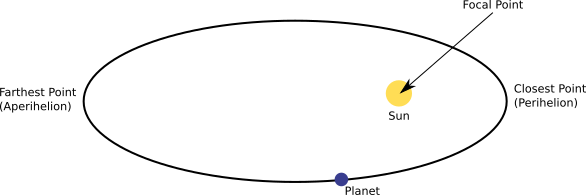
\includegraphics[width=0.8\textwidth]{figs/chapt-13/kepler-1.png}
\end{center}
  \caption{Kepler's First Law}
  \label{kepler-1}
\end{figure}

Of course, it looks nothing like this -- this is MASSIVELY exaggerated
for the sake of seeing what is going on. The Earth's orbit around the
Sun is very nearly circular, which is why it took so long for
astronomers to realise that it wasn't.

\subsection{Second Law}

\begin{figure}[h]
  \begin{center}
    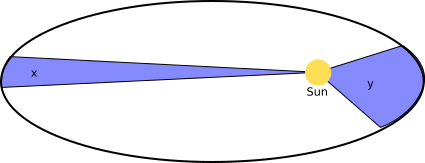
\includegraphics[width=0.8\textwidth]{figs/chapt-13/kepler-2.png}
  \end{center}
  \caption{Kepler's Second Law}
  \label{kepler-2}
\end{figure}

As you can see from the diagram, areas x and y are the same. The reason
for this, put simply, is that the objects move more quickly when they
are closer to the Sun and more slowly when they are further away.

\subsection{Third Law}

This will be described in more detail below.


\spec{recognise and use $F=-\frac{Gm_1m_2}{r^2}$}

``The gravitational force between two objects is proportional to the
product of their masses and inversely proportional to the square of the
distance between their centres.''

That is a lot of words and it is much more easily explained with an
equation:

\[F = - \frac{Gm_{1}m_{2}}{r^{2}}\]

Where: F is the force, measured in newtons (N)

G is the universal gravitational constant, which has a value of
6.67x10\textsuperscript{-11} Nm\textsuperscript{2}kg\textsuperscript{-2}

m\textsubscript{1} and m\textsubscript{2} are the two masses measured in
kilograms (kg)

r is the distance between their centres, measured in metres (m).

\begin{figure}[h]
  \begin{center}
    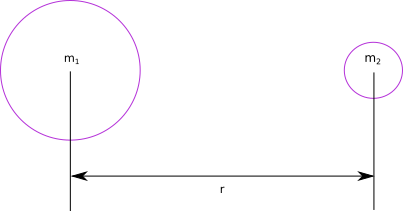
\includegraphics{figs/chapt-13/masses.png}
  \end{center}
  \label{masses}
  \caption{Two masses}
\end{figure}

Important things to note:

\begin{enumerate}
\def\labelenumi{\arabic{enumi}.}
\item
  The force is negative. This is because it is always attractive and
  attractive forces are always negative, by definition.
\item
  The force exerted by mass 1 on mass 2 is the same magnitude but
  opposite in direction to the force exerted by mass 2 on mass 1. This
  is a direct consequence of Newton's third law. In most cases that we
  study the \textbf{effect} of the force on the smaller mass is much
  greater than it is on the larger mass and we ignore the effects of the
  force on the larger mass.
\end{enumerate}



\spec{use Newton’s law of gravity and centripetal force to derive $ r^3 \propto T^2 $for a circular orbit}

Now that we know the size of the force acting on a body moving in
circular motion due to the gravitational force acting on it, we can
prove Kepler's third law:

For a body orbiting another body, the centripetal force is provided by
the gravitational force.

\[F = - \frac{Gm_{1}m_{2}}{r^{2}}\ \ (1)\]

As the body is moving in circular motion, the gravitational force causes
the body to accelerate towards the centre of the circle, as in the
diagram:

\begin{figure}[h]
  \begin{center}
    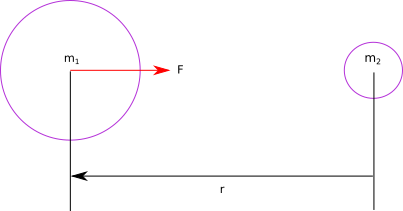
\includegraphics{figs/chapt-13/masses-direction.png}
  \end{center}
  \label{masses-2}
  \caption{Two masses and a force}
\end{figure}

Thus we apply F=ma, with F being the gravitational force, as on the
diagram, and the acceleration being equal to rω\textsuperscript{2}.

\[F = ma\]

So \[G\frac{m_{1}m_{2}}{r^{2}} = m_{1}r\omega^{2}\]

m\textsubscript{1} is the object that is orbiting, so it is the mass of
m\textsubscript{1} that is feeling the acceleration and thus
m\textsubscript{1} goes into the right hand side of the equation.

Thus we can cancel m\textsubscript{1} and collect the terms in r to
give:

\[Gm_{2} = r^{3}\omega^{2}\ \ (2)\]

But we know from our revision of circular motion that the period of the
orbit is related to the angular velocity by:

\[\omega = \frac{2\pi}{T}\ \ (3)\]

Therefore we substitute equation (3) into equation (2) to give:

\[Gm_{2} = \frac{{4\pi^{2}r}^{3}}{T^{2}}\]

Now re-arrange to make r the subject of the formula:

\[r^{3} = \frac{Gm_{2}}{{4\pi}^{2}}T^{2}\ \ (4)\]

G, m\textsubscript{2} and π are all constants, so we can finally write:

\[r^{3} \propto T^{2}\]

You need to be able to do this for your examination, so make sure that
you learn this proof.

\spec{understand energy transfer by analysis of the area under a gravitational force-distance graph}

Later you learned that in fact it was the area under the Force-distance
graph.

\emph{(Of course, it's a little bit more difficult than that. It is
actually given by:}

\[Work\ done = \int_{r}^{\infty}{F{dx\ \ \ \ (8)}}\]

\emph{You use this integral in other parts of the specification, but not
this part.)}

Therefore if we want to know the gravitational potential energy gained
or lost by an object in a gravitational field, we look at the area under
the force-distance graph.

The zero of gravitational potential energy is taken as being at
infinity, which makes sense. If the object isn't in a field, then it
isn't experiencing any force, so it doesn't have any GPE.

This does mean, however, that all gravitational potential energies are
negative as they lose GPE as they fall towards a mass.

For example, if you want to know the GPE gained/lost by an object as it
moves from point $R_1$ to point $R_2$ in the field you look at the area under
the force-distance graph (see figure \ref{gpe-area})

\begin{figure}
  \begin{center}
  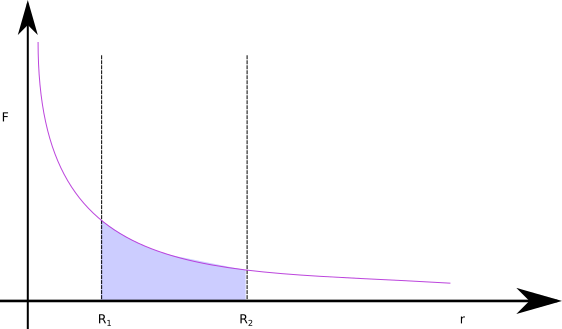
\includegraphics[width=0.8\textwidth]{figs/chapt-13/area-energy.png}
\end{center}
  \caption{Graviational PE as area of a graph}
  \label{gpe-area}
\end{figure}


\emph{(Generally, we tend to look at the gravitational potential rather
than the GPE, and use the field strength-distance graph, but the
specification asks for GPE and a force-distance graph, so that is what
we are looking at!)}

\spec{derive and use $g = -\frac{Gm}{r^2}$for the magnitude of the gravitational field strength due to a point mass}

If you look back to chapter 2 on gravitational fields, you will know the
definition of the gravitational field strength. It is given by the
equation:

\[g = \frac{F}{m}\ \ (5)\]

But we now know how the force is provided by a spherical mass from
Newton's Law of Gravitation. It is given by equation (1) as:

\[F = \frac{Gm_{1}m_{2}}{r^{2}}\ \ (6)\]

So we can substitute equation (6) into equation (5) to give us:

\[g = \frac{\text{Gm}}{r^{2}}\ \ (7)\]

This is the gravitational field strength due to a spherical mass m at a
distance r from its centre and you need to be able to derive this
equation.

A graph of the field strength due to a spherical body against distance
looks like this:

\begin{figure}[h]
  \begin{center}
  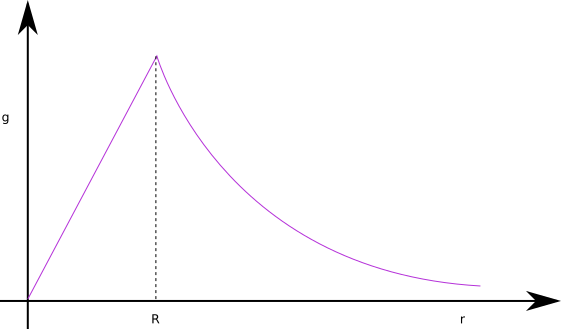
\includegraphics[width=0.8\textwidth]{figs/chapt-13/g-r.png}
\end{center}
  \caption{Field strength due to a sphere}
  \label{}
\end{figure}

From the centre of the object up to its radius (0 to R) the variation
with field strength inside the body varies linearly \textbf{if the
density is constant.} R is the radius of the body, so therefore the
distance from the centre. After R it drops off as
1/r\textsuperscript{2}.
\newpage
\spec{recall similarities and differences between electric and gravitational fields}

\begin{figure}[h]
  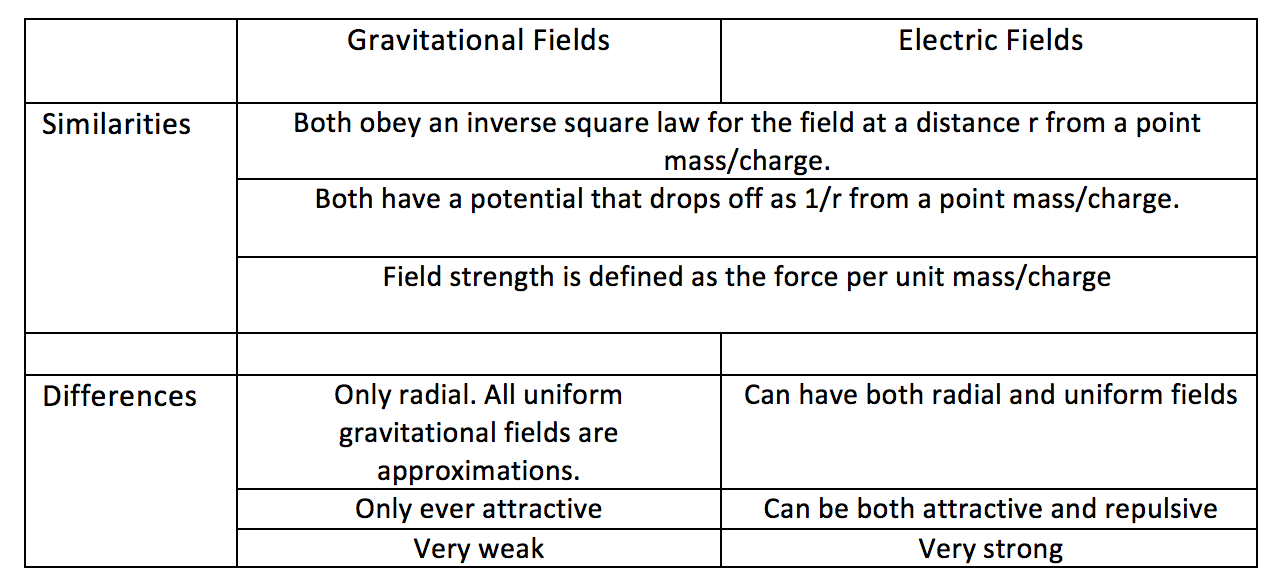
\includegraphics[width=\textwidth]{figs/chapt-13/table.png}
  \caption{Similarities and Differences}
  \label{tab:sim}
\end{figure}

\spec{recognise and use the equation for gravitational potential energy for point masses $ E = - \frac{Gm_1m_2}{r}$}

There is an equation for the GPE which you need to be able to use. It is
found from integrating the expression for the force as mentioned
earlier, and it is given by:

\[E = - \frac{Gm_{1}m_{2}}{r}\ \ \ \ (9)\]

\spec{calculate escape velocity using the ideas of gravitational potential energy (or area under a force-distance graph) and energy transfer}

We can now use these methods of working out the GPE gained by an object
in a gravitational field to calculate a quantity called the
\textbf{escape velocity.}

NB. A lot of people get escape velocity wrong. It is the velocity needed
to be given to an object \textbf{on the surface of the planet} in order
for it to escape the gravitational field of the planet and have zero KE
at that time. Once it has been given this velocity (by, for example, a
cannon) \textbf{no more energy is put into the system}. From that moment
on it is a projectile and is constantly losing KE as it gains GPE.

Of course, this means that when it finally escapes the gravitational
field it has no energy at all, which also means that it has zero overall
energy to start with as well!

Therefore we use the law of conservation of energy to work out what the
escape velocity must be:

Total energy before = Total energy after = 0

Therefore Initial KE + Initial GPE = 0

\[\frac{1}{2}mv_{e}^{2} - \frac{\text{GMm}}{R} = 0\ \ \ \ \left( 10 \right)\]

Where M is the mass of the planet in kg

R is the radius of the planet in m

m is the mass of the projectile in kg

v\textsubscript{e} is the escape velocity in ms\textsuperscript{-1}

You can cancel the mass of the projectile and re-arrange for
v\textsubscript{e} from equation (10) to give:

\[v_{e} = \sqrt{\frac{2GM}{R}}\ \ \ \ \ (11)\ \ \]

This is the escape velocity and you can work it out for the Earth. You
should get about 12 kms\textsuperscript{-1}.

There is a graphical way of looking at this as well. The GPE gained by
the body as it moves from the surface of the planet, radius R, is given
by the area under the force-distance graph from the surface of the
planet to infinity. If it is launched from the surface of the planet
then that also equals its initial KE.

\spec{calculate the distance from the centre of the Earth and the height above its surface required for a geostationary orbit.}

A geostationary orbit is one which stays above the same position on the
Earth's equator at all times.

This means, therefore, that it has a period of 24 hours.

It is therefore possible to calculate, using equation (4), r for a
geostationary orbit.

N.B. A very common mistake is to say that r is the height of the orbit.
This isn't the case -- it is the radius of the orbit, so it is the
distance of the satellite from the \textbf{centre} of the Earth, not the
surface of the Earth.

You should make sure that you can do this. Have a go at working out r,
given the following data:

G = 6.67 x 10\textsuperscript{-11}
Nm\textsuperscript{2}kg\textsuperscript{-2}

M\textsubscript{E} = 5.98 x 10\textsuperscript{24} kg

and remembering that T = 24 hours (but don't forget to convert to
seconds!)

You should have got an answer of 4.23 x 10\textsuperscript{7} m.

If I now tell you that the radius of the Earth is
6.36 x 10\textsuperscript{6} m, you can also write down the height of the
satellite above the surface of the Earth, and this comes to
3.6 x 10\textsuperscript{6} m.

So a geostationary satellite orbits at a height that is about 6 times
greater than the radius of the Earth.
\end{document}
